\documentclass[12pt, letterpaper]{article}
\usepackage[margin=1in]{geometry}
\usepackage{amsmath,amsthm,array, amssymb,amsfonts, enumitem, fancyhdr, color, comment, graphicx, environ}

\setlist[description]{leftmargin=\parindent,labelindent=\parindent}

\author{Val Anthony Balagon}
\date{January 2019}
\title{Chapter 4: Orthogonality}

%User commands
\newcommand{\R}[1]{$\mathbb{R}^{#1}$}
\newcommand{\Vector}[1]{$\textbf{#1}$}
\newcommand{\V}[1]{\textbf{\textit{#1}}}

\newcommand{\A}{$A$}
\newcommand{\x}{\textbf{\textit{x}}}
\newcommand{\B}{\textbf{\textit{b}}}
\newcommand{\system}{\textbf{\textit{\A \x = \B}}}
\newcommand{\nullsystem}{\textbf{\textit{\A\x}} = \textbf{0}}
\newcommand{\DefinitionSpace}{\vspace{15px}}


\newtheorem*{remark}{Remark}
\theoremstyle{definition}
\newtheorem{definition}{Definition}[section]
\newtheorem{example}{Example}
\newtheorem{theorem}{Theorem}

\newcommand*{\vertbar}{\rule[-1ex]{0.5pt}{2.5ex}}



\newenvironment{problem}[2][Problem]{\begin{trivlist}
		\item[\hskip \labelsep {\bfseries #1}\hskip \labelsep {\bfseries #2.}]}{\end{trivlist}}



\begin{document}
	\maketitle
	\begin{abstract}
		This chapter focuses on the orthogonality of the four subspaces, projections, and least squares approximations.
	\end{abstract}

\section{Orthogonality of the Four Subspaces}

	Two vectors are orthogonal when their dot product is zero $\V{v} \cdot \V{w} = \V{v}^T \V{w} = 0$. This chapter will revolve around orthogonal subspaces, orthogonal bases, and orthogonal matrices.
	
	\DefinitionSpace
	\begin{definition}
		Orthogonal vectors have the following properties:
		\renewcommand{\theenumi}{\roman{enumi}}
		
		\begin{enumerate}[leftmargin=2\parindent]
			\item $\V{v}^T \V{w} = 0$
			\item $||\V{v}||^2 + ||\V{w}||^2 = ||\V{v} + \V{w}||^2 \rightarrow \V{v}^T\V{v} + \V{w}^T\V{w} = (\V{v}+\V{w})^T(\V{v}+\V{w})$
		\end{enumerate}	
	
	\end{definition} 	
	
	\DefinitionSpace
	\begin{remark}
		The zero vector is orthogonal to any vector.
	\end{remark}
	

	\DefinitionSpace
	\begin{remark}
		The subspaces have orthogonal properties. 
		\begin{enumerate}
			\item \textbf{The rowspace $C(A^T)$ is perpendicular to the nullspace $N(A)$}. Every row of $A$ is perpendicular to the solution of $A\V{x} = \textbf{0}$.
			\item \textbf{The column space $C(A)$ is perpendicular to the left nullspaces $N(A^T)$}. When $\V{b}$ is outside of the column space when we're trying to solve for $A\V{x} = \V{b}$, then this nullspace of $A^T$ comes into its own. It contains the error $\V{e} = \V{b} - A\V{x}$ in the least-squares solution.
		\end{enumerate}
	\end{remark}
	\DefinitionSpace
	

	\begin{definition}
		Two subspaces \V{V} and \V{W} of a vector space are orthogonal if every vector \V{v} in \V{V} is perpendicular to every vector \V{w} in \V{W}.
		\renewcommand{\theenumi}{\roman{enumi}}
		
		\begin{equation*}
			\V{v}^T \V{w} = 0 \text{ for all \V{v} in \V{V} and all \V{w} in \V{W}.}
		\end{equation*}
	\end{definition} 	
	\DefinitionSpace
	
	
	\begin{theorem}
	Every vector \V{x} in the nullspace is perpendicular to every row of $A$, because $A\V{x} = \textbf{0}$. The nullspace $N(A)$ and the row space $C(A^T)$ are orthogonal subspaces of \R{n}.
	
		\begin{equation*}
			A \V{x} = \begin{bmatrix} \text{row 1} \\ \vdots \\ \text{row m} \end{bmatrix} \begin{bmatrix} x_1 \\ \vdots \\ x_n \end{bmatrix} = \begin{bmatrix} 0 \\ \vdots \\ 0 \end{bmatrix}
		\end{equation*}
		\begin{gather*}
			C_1(\text{row}_1^T) = 0 \\
			C_2(\text{row}_2^T) = 0 \\
			\vdots \\
			C_m(\text{row}_m^T) = 0
		\end{gather*}
	\end{theorem}
	\noindent (row 1) $\cdot \V{x}$ is zero and (row $m) \cdot \V{x}$ is also zero. Every row has a zero dot product with \V{x}. Then \V{x} is perpendicular to every combination of the rows. \textbf{The whole row space $C(A^T)$ is orthogonal to $N(A)$. }
	\DefinitionSpace
	
	
	\begin{proof}
		The vectors in the row space are combinations of $A^T \V{y}$ of the rows. We take the dot product of $A^T \V{y}$ with any \V{x} in the nullspace.
			\begin{gather*}
				\V{x} \cdot (A^T \V{y}) = \V{x}^T (A^T \V{y}) = (A\V{x})^T \V{y} = 0^T \V{y} = 0
			\end{gather*}
	\end{proof}
	\DefinitionSpace
	
	\begin{example}
		The rows of $A$ are perpendicular to $\V{x} = (1,1,-1)$ in the nullspace:
		\begin{gather*}
			A\V{x} = \begin{bmatrix} 1&3&4 \\ 5&2&7\end{bmatrix} \begin{bmatrix} 1 \\ 1 \\ -1 \end{bmatrix} = \begin{bmatrix} 1+3-4 \\ 5+2-7 \end{bmatrix} = \begin{bmatrix} 0\\ 0 \end{bmatrix}
		\end{gather*}
		In this example, the column space is all of \R{2}. The nullspace of $A^T$ is the zero vector. The column space of $A$ and the nullspace of $A^T$ are always orthogonal subspaces.
	\end{example}


	\begin{theorem}
		Every vector \V{y} in the nullspace of $A^T$ is perpendicular to every column of $A$. The left nullspace $N(A^T)$ and the column space $C(A)$ are orthogonal in \R{m}.
	\end{theorem}

	\begin{proof}
		The nullspace of $A^T$ is orthogonal to the row space of $A^T$, which is the column space of $A$.
		
		\begin{gather*}
			A^T\V{y} = \begin{bmatrix} \text{(column 1)}^T \\ \vdots \\ \text{(column n)}^T \end{bmatrix} \begin{bmatrix} y_1 \\ \vdots \\ y_m \end{bmatrix} = \begin{bmatrix} 0 \\ \vdots \\ 0 \end{bmatrix}
		\end{gather*}
	\end{proof}
	
	\DefinitionSpace
	\begin{theorem}
		If a vector \V{v} is orthogonal to itself, then \V{v} is the zero vector.
	\end{theorem}
	\DefinitionSpace
	
	\begin{figure}[h!]
		\centering
		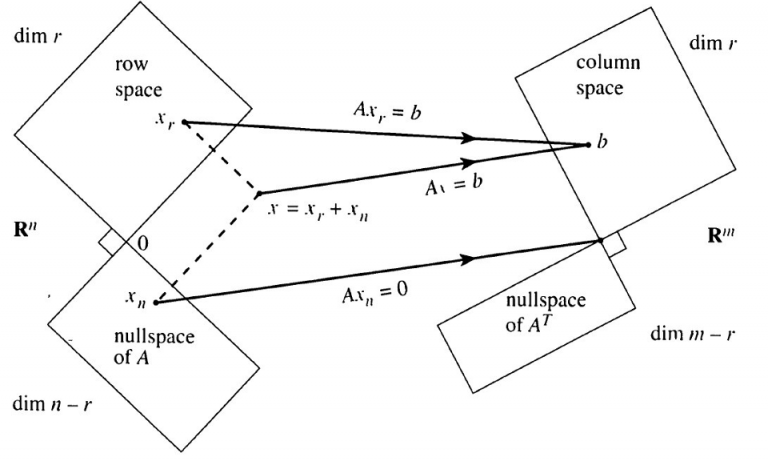
\includegraphics[scale=0.5]{4-subspaces.png}
		\caption{The Four Subspaces. There are two pairs of orthogonal subspaces.}
		\label{4subs}
	\end{figure}

	\begin{theorem}
		Fundamental Theorem of Linear Algebra, Part 2: \\
		\quad\textbf{$N(A)$ is the orthogonal complement of the row space $C(A^T)$ in \R{n}. \\
		\quad $N(A^T)$ is the orthogonal complement of the column space $C(A)$ in \R{m}.}
	\end{theorem}\DefinitionSpace 

	Things to note from Figure \ref{4subs}
	\begin{enumerate}
		\item When $A$ multiplies to $\V{x} = \V{x}_r + \V{x}_n$, it goes to \V{b} which is in the column space.
		\item When $A$ multiplies to $\V{x}_r$, it goes to \V{b} which is also in the column space.
		\item When $A$ multiplies to $\V{x}_n$, the nullspace component goes to \textbf{0}.
	\end{enumerate}
	
	
	
\subsection{Combining Bases from Subspaces}
	\begin{theorem}
		Any independent vectors in \R{n} must span \R{n}. So they are a basis.\\
		Any $n$ vectors that span \R{n} must be independent. So they are a basis
	\end{theorem}\DefinitionSpace 
	
	\begin{theorem}
		If the $n$ columns of $A$ are independent, they span \R{n}. So $A\V{x} = \V{b}$ is solvable.\\
		If the $n$ columns span \R{n}, they are independent. So $A\V{x} = \V{b}$ has only one solution.
	\end{theorem}\DefinitionSpace 
	
	
	
\section{Projections}
	Let's say we are given an arbitrary vector \V{b}. When \V{b} is projected onto a line, its projection \V{p} is the part of \V{b} along that line. If \V{b} is projected onto a plane, \V{p} is a part in that plane. The projection \V{p} is $P\V{b}$. The projection matrix $P$ multiplies \V{b} to give \V{p}.
	
	\begin{figure}[h!]
		\centering
		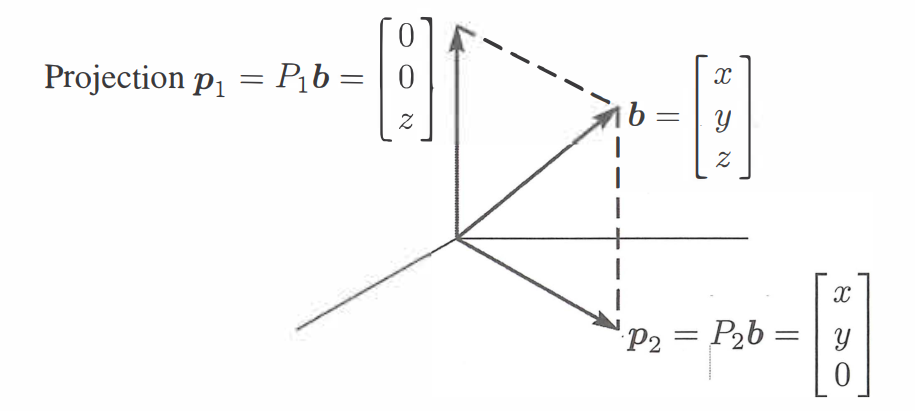
\includegraphics[scale=0.5]{projection.png}
		\caption{The projections $\V{p}_1$ and $\V{p}_2$ onto the $z$ axis and the $xy$ plane.}
		\label{projection}
	\end{figure}
	
	Say $\V{b} = \begin{bmatrix} 2 & 3 & 4\end{bmatrix}^T$, its projections are $\V{p}_1=\begin{bmatrix} 0 & 0 & 4\end{bmatrix}^T \text{and} \V{p}_2=\begin{bmatrix} 2 & 3 & 0\end{bmatrix}^T$ in Figure \ref{projection}. $\V{p}_1 \text{and} \V{p}_2$ are the projections of \V{b} onto the $z$ axis and $xy$ axis, respectively. The projection matrices $P_1$ and $P_2$ are $3 \times 3$ matrices. Projection onto a line comes from a rank one matrix, while a projection onto a planes comes from a rank two matrix.
	
		\begin{gather*}
			\text{Onto the $z$ axis: }P_1 = \begin{bmatrix} 0 & 0 & 0 \\ 0 & 0 & 0 \\ 0 & 0 & 1 \end{bmatrix} \qquad \text{Onto the $xy$ plane: }P_2 = \begin{bmatrix} 1 & 0 & 0 \\ 0 & 1 & 0 \\ 0 & 0 & 0 \end{bmatrix}  \\
			\V{p}_1 = P_1\V{b} = \begin{bmatrix} 0 & 0 & 0 \\ 0 & 0 & 0 \\ 0 & 0 & 1 \end{bmatrix} \begin{bmatrix} 2\\3\\4 \end{bmatrix} = \begin{bmatrix} 0 \\ 0 \\ 4 \end{bmatrix} \qquad \V{p}_2 = P_2\V{b} = \begin{bmatrix} 1 & 0 & 0 \\ 0 & 1 & 0 \\ 0 & 0 & 0 \end{bmatrix} \begin{bmatrix} 2\\3\\4 \end{bmatrix} = \begin{bmatrix} 2 \\ 3 \\ 0 \end{bmatrix}
		\end{gather*}

	The projections $p_1$ and $p_2$ are perpendicular. The $xy$ plane and the $z$ axis are orthogonal subspaces. The line and plane are also orthogonal complements. Their dimensions add to $1+2=3$. Every vector \V{b} in the whole space is the sum of its parts in the two subspaces. The projections $\V{p}_1 \text{and} \V{p}_2$ are exactly those two parts of \V{b}:
		\begin{gather*}
			\text{The vectors give } \V{p}_1 + \V{p}_2 = \V{b} \qquad \text{The matrices give } P_1 + P_2 = I 
		\end{gather*}
	
	
	
	In general, the objective is to find \V{p} in each subspace, and the projection matrix $P$ that produces that part $\V{p} = P\V{b}$. Every subspace of \R{m} has its own $m\times m$ projection matrix. To compute $P$, we need a good description of the subspace that it projects onto. The best description of a subspace is a basis. We put the basis vectors into the columns of $A$. Now we are projecting onto the column space of A. The problem now is to project any \V{b} onto the column space of any $m \times n$ matrix.
	
	
\subsection{2-D Case}
		\begin{figure}[h!]
			\centering
			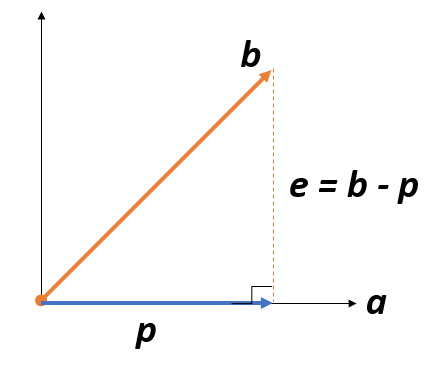
\includegraphics[scale=0.5]{projection_2D.png}
			\caption{The projection of \V{b} onto \V{a}}
			\label{projection2D}
		\end{figure}
	
	A line goes through the origin in the direction \V{a}. Along that line, we want the point \V{p} closest to \V{b}. The key to projection is orthogonality: The line from \V{b} to \V{p} is perpendicular to the vector \V{a}. This is the dotted line marked $\V{e} = \V{b} - \V{p}$ for the error on the left side of Figure \ref{projection2D}. We now comute \V{p} by algebra. 
	
	The projection \V{p} will be a multiple of \V{a}. We call it $\V{p} = \hat{\V{x}} \V{a}$. Computing this number $\hat{\V{x}}$ will give the vector \V{p}. Then from the formula \V{p}, we will read off the projection matrix $P$. These three steps will lead to all projection matrices: \textbf{find $\hat{\V{x}}$, then find the vector \V{p}, then fin the matrix \V{P}}.

		\begin{gather*}
			\intertext{Projecting \V{b} onto \V{a} with error $\V{e} = \V{b} - \hat{\V{x}}\V{a}$:}
				\V{a} \cdot (\V{b} - \hat{\V{x}}\V{a}) = 0 \text{\quad or \quad} \V{a} \cdot \V{b} - \hat{\V{x}}\V{a} \cdot \V{a} = 0  \\
				\hat{\V{x}} = \frac{\V{a} \cdot \V{b}}{\V{a} \cdot \V{a}} = \boxed{\frac{\V{a}^T\V{b}}{\V{a}^T\V{a}}}
		\end{gather*}

		
		\begin{theorem}
			The projection of \V{b} onto the line through \V{a} is the vector $\V{p} = \hat{\V{x}}\V{a} = \frac{\V{a}^T\V{b}}{\V{a}^T\V{a}} \V{a}$
				\begin{description}
					\item[Special Case 1:] If $\V{b} = \V{a}$, then $\hat{\V{x}} = 1$. The projection of $\V{a}$ onto $\V{a}$ is itself. $P\V{a} = \V{a}$.  
					\item[Special Case 2:] If \V{b} is perpendicular to \V{a}, then $\V{a}^T \V{b} = 0$. The projection is $\V{p} = 0$.
				\end{description}
		\end{theorem}\DefinitionSpace 


	\begin{example}
		Project $\V{b} = \begin{bmatrix} 1 \\ 1 \\ 1 \end{bmatrix}$ onto $\V{a} = \begin{bmatrix} 1 \\ 2 \\ 2 \end{bmatrix}$ to find $\V{p} = \hat{\V{x}}\V{a}$.
			\begin{gather*}
				\V{p} = \hat{\V{x}}\V{a} = \frac{\V{a}^T\V{b}}{\V{a}^T\V{a}} \V{a} = \frac{\begin{bmatrix} 1 & 2 & 2 \end{bmatrix}\begin{bmatrix} 1 \\ 1 \\ 1 \end{bmatrix}}{\begin{bmatrix} 1 & 2 & 2 \end{bmatrix} \begin{bmatrix} 1 \\ 2 \\ 2 \end{bmatrix}} \V{a} = \boxed{\frac59 \V{a}}
			\intertext{The error vector between \V{b} and \V{p} is $\V{e} =\V{b} - \V{p}$. Those vectors \V{p} and \V{e} will add to \V{b}=$\begin{bmatrix} 1 \\ 1 \\ 1 \end{bmatrix}$}
				\V{p} = \left(\frac59, \frac{10}{9},\frac{10}{9} \right) \qquad \text{and\qquad} \V{e} = \V{b} - \V{p} =  \left(\frac49, -\frac19, -\frac19 \right)
			\intertext{To get the magnitude of $\V{p}$:}
				||\V{p}|| = \frac{||\V{a}|| ||\V{b}||\cos{\theta}}{||\V{a}||^2}||\V{a}|| = ||\V{b}|| \cos{\theta}
			\intertext{Now to find the projection matrix,}
				\V{p} = \V{a} \hat{\V{x}} = \V{a} \frac{\V{a}^T \V{b}}{\V{a}^T \V{a}} = P\V{b} \text{ then } P = \frac{\V{a}\V{a}^T}{\V{a}^T \V{a}} \\
				P = \begin{bmatrix}
					\frac19 & \frac29 & \frac29\\
					\frac29 & \frac49 & \frac49\\
					\frac29 & \frac49 & \frac49
					\end{bmatrix}
			\intertext{$P$ is a column times a row! Then column is \V{a}, the row is $\V{a}^T$. Then divide by the number $\V{a}^T\V{a}$. The projection matrix $P$ is an $m \times m$ matrix, but its rank is 1. We are projecting onto a 1-D subspace, a line through \V{a}. \textit{That line is the column space of $P$}. Next, we try to project a second time.}
				P^2 = \begin{bmatrix}
						\frac19 & \frac29 & \frac29\\
						\frac29 & \frac49 & \frac49\\
						\frac29 & \frac49 & \frac49
						\end{bmatrix} \begin{bmatrix}
										\frac19 & \frac29 & \frac29\\
										\frac29 & \frac49 & \frac49\\
										\frac29 & \frac49 & \frac49
										\end{bmatrix} = \begin{bmatrix}
														\frac19 & \frac29 & \frac29\\
														\frac29 & \frac49 & \frac49\\
														\frac29 & \frac49 & \frac49
														\end{bmatrix} = P \\
				\boxed{P^2 = P}
			\intertext{Notice that projecting a second time does not change anything. Notice also that $P$ is symmetric.}
			\end{gather*}
	\end{example}\DefinitionSpace 

	\noindent To summarize:
		\begin{enumerate}
			\item $C(P)$ is a line through $A$
			\item $\text{rank}(P)$ = 1
			\item $P^T = P$, $P$ is symmetric
			\item $P^2 = P$, projecting a second time does not change anything
		\end{enumerate}

\subsection{Projection Onto A Subspace}
	We now move to $n$ vectors $a_1, \ldots,a_n$ in \R{m}. We assume that these \V{a}'s are linearly independent. The problem now becomes: how do we find the combination $\V{p} = \hat{\V{x}_1}a_1 + \ldots + \hat{\V{x}_n}a_n$ closest to a given vector \V{b}? We are projecting \V{b} in \R{m} onto the subspace spanned by the $\V{a}$'s.
	
	We compute projections onto $n$-dimensional subspaces in three steps as before: \textbf{\textit{Find a vector $\hat{\V{x}}$, find the projection $\V{p} = A \hat{\V{x}}$, find the projection matrix $P$.}}
	
		\begin{figure}[h!]
			\centering
			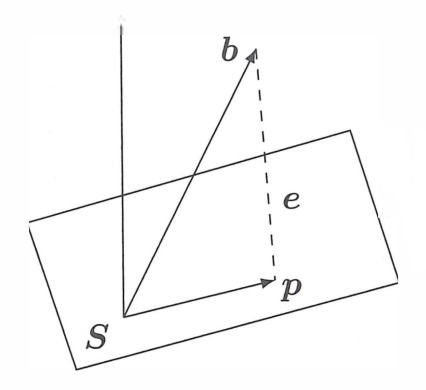
\includegraphics[scale=0.5]{projection_n.png}
			\caption{The projection \V{p} of \V{b} onto $\V{S}$ = column space of $A$}
			\label{projection_n}
		\end{figure}
	
	The error vector $\V{b} - A\hat{\V{x}}$ is perpendicular to the subspace. In $n$-dimensions, there will be $n$ equations for $\hat{\V{x}}$. The error makes a right angle with all the vectors $a_1, \ldots, a_n$ in the base. The $n$ right angles give the $n$ equations for $\hat{\V{x}}$.
		\begin{gather}
			\begin{bmatrix}
			\rule{0.5cm}{0.001em} & a_1^T & \rule{0.5cm}{0.001em} \\
			&\vdots& \\ 
			\rule{0.5cm}{0.001em} & a_n^T & \rule{0.5cm}{0.001em} 
			\end{bmatrix}
		\end{gather}
	
	\begin{gather}
		\intertext{The combination $\V{p} = \hat{x_1}\V{a}_1 + \ldots + \hat{x_n}\V{a}_n = A \hat{\V{x}}$ that is closest to \V{b} comes from $\hat{\V{x}}$:}
		\boxed{	A^T(\V{b} - A\hat{\V{x}}) = \textbf{0}} \qquad\text{or \qquad} \boxed{A^TA\hat{\V{x}} = A^T \V{b}}
		\intertext{This symmetric $A^T A$ is $n \times n$. It is invertivle if $\V{a}$'s are independent. The solution $\hat{\V{x}} = (A^T A)^{-1} A^T \V{b}$. The projection of \V{b} onto the subspace is \V{p}:}
			\boxed{\V{p} = A\hat{\V{x}} = A(A^T A)^{-1} A^T \V{b}}
		\intertext{To find the projection matrix $P$:}
			\boxed{P = A(A^TA)^{-1} A^T}
	\end{gather}

	The equations above are equivalent to their $n = 1$ counterparts. We use the inverse $(A^T A)^{-1}$ instead of $\frac{1}{\V{a}^T\V{a}}$. Matrix inversion is a guarantee because the columns of $A$ are linearly independent.
	
	\noindent Here are interesting properties:
		\begin{enumerate}
			\item Our subspace is the column space of $A$
			\item The error vector $\V{b} - A\hat{\V{x}}$ is perpendicular to that column space
			\item Therefore $\V{b} - A\hat{\V{x}}$ is in the nullspace of $A^T$. This means that $A^T(\V{b} - A\hat{\V{x}})=\textbf{0}$ 
		\end{enumerate}

	\begin{example}
		If $A = \begin{bmatrix} 1 & 0\\ 1 & 1 \\ 1&2 \end{bmatrix}$ and $\V{b} = \begin{bmatrix} 6 \\ 0 \\ 0 \end{bmatrix}$ find $\hat{\V{x}}$ and $\V{p}$.
		\begin{gather*}
		\intertext{Computing for $A^T A$ and $A^T \V{b}$}
			A^T A = \begin{bmatrix} 1 & 1 & 1\\ 0 & 1 & 2 \end{bmatrix} \begin{bmatrix} 1 & 0\\ 1 & 1 \\ 1&2 \end{bmatrix} = \begin{bmatrix}
																																3 & 3 \\
																																3 & 5
																																\end{bmatrix} \\
			A^T \V{b} = \begin{bmatrix} 1 & 1 & 1\\ 0 & 1 & 2 \end{bmatrix} \begin{bmatrix} 6 \\ 0 \\ 0 \end{bmatrix} = \begin{bmatrix}6 \\ 0\end{bmatrix} \\
		\intertext{Computing for $\hat{\V{x}}$}
			\begin{bmatrix}
			3 & 3 \\
			3 & 5
			\end{bmatrix} \begin{bmatrix} \hat{x}_1 \\ \hat{x}_2 \end{bmatrix} = \begin{bmatrix}6 \\ 0\end{bmatrix} \rightarrow \hat{\V{x}} = \begin{bmatrix} \hat{x}_1 \\ \hat{x}_2 \end{bmatrix} = \begin{bmatrix}5 \\ -3\end{bmatrix}
		\intertext{Finding $\V{p}$:}
			\V{p} = \begin{bmatrix} 1 & 0\\ 1 & 1 \\ 1&2 \end{bmatrix} \begin{bmatrix}5 \\ -3\end{bmatrix} = \begin{bmatrix} 5 \\ 2\\-1 \end{bmatrix} 
		\intertext{Finding the error:}
			\V{e} = \V{b} - \V{p} = \begin{bmatrix} 1 \\ -2 \\ 1 \end{bmatrix} 
		\intertext{Finding $P$:}
			(A^T A)^{-1} = \frac{1}{6} \begin{bmatrix} 5 & -3 \\ -3 & 3\end{bmatrix} \\
			P = A(A^TA)^{-1} A^T = \begin{bmatrix} 1 & 0\\ 1 & 1 \\ 1&2 \end{bmatrix} * \frac{1}{6} \begin{bmatrix} 5 & -3 \\ -3 & 3\end{bmatrix}  * \begin{bmatrix} 1 & 1 & 1\\ 0 & 1 & 2 \end{bmatrix} = \frac{1}{6} \begin{bmatrix} 5 & 2 & -1\\ 2 & 2 & 2 \\ -1 & 2 & 5\end{bmatrix}
		\intertext{Projecting it twice,}
			P^2 = \frac{1}{6} \begin{bmatrix} 5 & 2 & -1\\ 2 & 2 & 2 \\ -1 & 2 & 5\end{bmatrix} * \frac{1}{6} \begin{bmatrix} 5 & 2 & -1\\ 2 & 2 & 2 \\ -1 & 2 & 5\end{bmatrix} = \frac{1}{6} \begin{bmatrix} 5 & 2 & -1\\ 2 & 2 & 2 \\ -1 & 2 & 5\end{bmatrix} \\
			P^2 = P
		\end{gather*}
	\end{example}\DefinitionSpace 

	If $A$ is a rectangular matrix, then we won't be able to do $(A^T A)^{-1}=A^{-1} (A^T)^{-1}$. This is because $A$ does not have an inverse.
	
		\begin{theorem}
			$A^T A$ is invertible if and only if $A$ has linearly independent columns.
		\end{theorem}\DefinitionSpace 

		\begin{theorem}
			When $A$ has independent columns, $A^T A$ is square and invertible.
		\end{theorem}
		\begin{proof}
			\begin{gather*}
				\intertext{Take the transpose of $A^T A$:}
					(A^T A)^T = A^T (A^T)^T = A^T A \\
					(A^T A)^T = A^T A
			\end{gather*}
			Hence, $A^T A$ is symmetric. Since $A$ has independent columns, this means that $A^T$ is also invertible. Hence, $A^T A$ is invertible.
		\end{proof}










\section{Least Squares Approximations}





\section{Orthonormal Bases and Gram-Schmidt}




\section{Problems}


	\begin{problem}{1.1}
		asd
	\end{problem}
	
	\begin{proof}[Solution]
		soln
	\end{proof}
	
	
	
	
	
	
	


\end{document}